\subsection{Pyramid}
\begin{figure}[h]
	\begin{subfigure}{0.5\textwidth}
		\centering
		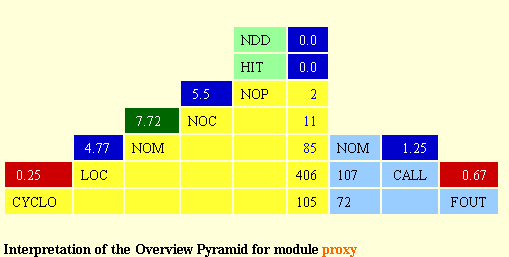
\includegraphics[width=0.9\linewidth]{../Diagrams/pyramidPreRefactoringNoInfo}
		\caption{Pyramid before refactoring}
	\end{subfigure}%
	\begin{subfigure}{0.5\textwidth}
		\centering
		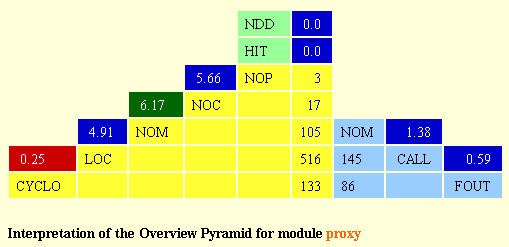
\includegraphics[width=0.9\linewidth]{../Diagrams/pyramidPostRefactoringNoInfo}
		\caption{Pyramid after refactoring}
	\end{subfigure}
	\caption{Pyramids of the org.parosproxy.paros.core.proxy package.}
\end{figure}

\begin{figure}[h]
	\begin{subfigure}{0.5\textwidth}
		\centering
		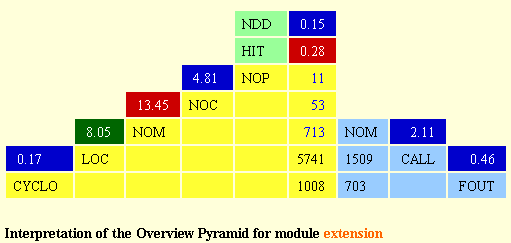
\includegraphics[width=0.9\linewidth]{../Diagrams/pyramidExtensionPreRef}
		\caption{Pyramid before refactoring}
	\end{subfigure}%
	\begin{subfigure}{0.5\textwidth}
		\centering
		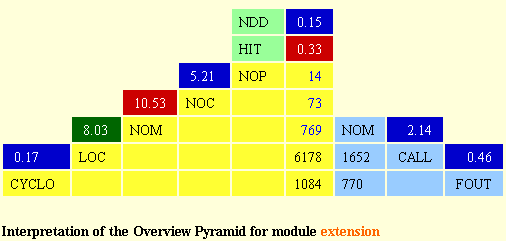
\includegraphics[width=0.9\linewidth]{../Diagrams/pyramidExtensionProstRef}
		\caption{Pyramid after refactoring}
	\end{subfigure}
	\caption{Pyramids of the org.parosproxy.paros.extension package.}
\end{figure}



\subsection{Test Coverage}
We only wrote JUnit tests for the 3rd iteration since others manipulate images.
First off we have a test \textit{testApplyBasicStringFilter}, which tests the basic functionality of our filter with some standard examples. 
Then we also wrote some tests that may be useful for future upgrades of our code.
The first future test \textit{testApplyBasicStringFilterCapitalLetters} tests whether certain words 
are also filtered out when they are partly in capital letters. 
The test \textit{testApplyBasicStringFilterWithWordsInBetween} checks if the filter still works if 
it needs to filter a combination of words and these words are not directly next to each other in a sentence.
\textit{testApplyBasicStringFilterWithChangedOrder} also applies to cases where it's a combination of
words that need to be filtered out, here we check if it's also filtered when the words are in a different 
ordering.
The test \textit{testApplyBasicStringFilterWithConjugatedVerbs} tests if the filter also detects the 
verb when it is conjugated.
Finally we have the test \textit{testApplyBasicStringFilterPartialCensoring} that checks if the filter detects 
partial cencoring. What we mean by this is when for example you need to filter the word "nigger" it also
detects the word n*gger.
